

\section{Numerical Experiments} \label{sec:res}

\subsection{Vortex Merging}
Consider the $2D$ incompressible Euler equation, \eqref{eq:3.8} with no viscous term, on a square domain $\Omega = [0,2\pi]^2$, provided with periodic boundary conditions. Spatial derivatives are discretized using a Fourier spectral method, which in centered differential operators in the Fourier space. To capture the fine details characterizing the solution, $256\times 256$ modes have been adopted. The initial condition is given in terms of the vorticity distribution $\mathbf{\omega} = \nabla \times u$ {\commnet \{ check this \}}. 

We consider the evolution of three different vortices, and the initial structure is given by
\begin{equation}\label{eqn:initial_cond_vort}
\omega = \omega_0 + \sum_{i=1}^{3} \alpha_i e^{-\dfrac{\left(x-x_i\right)^{2}+\left(y-y_i\right)^{2}}{\beta^2}}.
\end{equation}
In \eqref{eqn:initial_cond_vort}, $(x,y)$ represents the spatial coordinates, $\left( x_i, y_i\right)$ is the center of the $i$th vortex, $\alpha_i$ its maximum amplitude, and $\beta$ controls the effective radius of the vortex. In this example, the center of three vortices are positioned at 
\begin{equation}
\left( x_1, y_1 \right) = \left(0.75\pi,\pi\right) , \left( x_2, y_2 \right) = \left(1.25\pi,\pi\right), \left( x_3, y_3 \right) = \left(1.25\pi,1.5\pi\right),
\end{equation}
close to the center of the domain, of which, two have positive spins with $\alpha_1 = \alpha_2 = \pi$ and the other rotates in the opposite direction with $\alpha_3 = -0.5\pi$. The effective radius of all the vortices is set to $\beta = 1 / \pi$. This arrangement of vortices is an effective initial condition for the process of merging vortices. This phenomenon is often a result of fast-moving dipoles {\commnet \{ what is a dipole?\}} facing another vortex {\commnet \{ ref \}}. The forces developed in the merging process transfers the vorticity from the initial configuration, into long, narrow, and spiral-shaped strips of intense vorticity \cite{filaments_vort}. The formation of such thin vorticity filaments in the fluid, can pose numerical challenges. 

In the context of MOR, conservation of energy and stability is crucial for capturing fined structures, mentioned above. In the absence of natural dissipation, characterizing the Euler equation, straight forward application of MOR techniques is often unstable.

To define the initial conditions in terms of the velocity components $\omega$ and the pressure $p$, we define a stream-function $\Psi$, the solution to the equation 
\begin{equation} \label{eq:5.1}
	\nabla \Psi = \omega.
\end{equation}
The initial velocity is then given by $\nabla \times \Psi$. To solve the stream-function problem \eqref{eq:5.1}, we require $\int_{\Omega} \omega \ dx= 0$ {\commnet \{ check this \}}. It is easily verified that this requirement implies $\omega_0 = 0.038$. The pressure is recovered by solving the related Poisson pressure equation {\commnet \{ write the equation here \}}. The implicit midpoint scheme, to mimic the time integration scheme presented in \eqref{eq:3.27}, is considered to integrate in time. The merging phenomenon is simulated for a total of $18$ time units using a temporal step $\Delta t=0.004$.

\Cref{fig:unstable_full_models} illustrates the evolution of the kinetic energy for the advective, divergence, and the skew-symmetric form of the high-fidelity system. It is observed that only the skew-symmetric form preserves the kinetic energy, confirming the results in \Cref{sec:skew.2}.

%%%%%%%%%%%%%%%%%%%%%%%%%%%%%%%%%%%%%%%%%
%%%%% Comparison Skew symmetric, divergence and advective form %%%%%
%%%%%%%%%%%%%%%%%%%%%%%%%%%%%%%%%%%%%%%%%
\begin{figure}[t]
  \centering
  \begin{tikzpicture}[scale=0.5452]
    \begin{axis}[ylabel=$E_K(t)$,
                 xlabel=$t$,
                 label style={font=\large},
                 legend pos=south west,
                 legend entries={Skew Symmetric form, Divergent form, Advective form},
                 legend style={font=\large},
                 width=0.7\linewidth, 
                 height=0.5\linewidth,
                 minor x tick num=1,
                 minor y tick num=2,	
                 yticklabel style={/pgf/number format/.cd,fixed,precision=4},
                 scaled x ticks = true,
                 enlargelimits=false,
                 scale only axis]
                 \addplot[color=red,style=solid,style=ultra thick]  table[x = time, y = energy] {./data/Incompressible_Euler/Energy_compare_formulations/energy_skew_symmetric.txt};
                 \addplot[color=blue,style=solid,style=ultra thick]  table[x = time, y = energy] {./data/Incompressible_Euler/Energy_compare_formulations/energy_divergence.txt};
                 \addplot[color=black!50!green,style=solid,style=ultra thick]  table[x = time, y = energy] {./data/Incompressible_Euler/Energy_compare_formulations/energy_convective.txt};
    \end{axis}%  
  \end{tikzpicture}
  \caption{Conservation of the kinetic energy $K$ for the advective, divergence and the skew-symmetric formulations. {\commnet \{ please change Divergent to Divergence in the legend \}} }
  \label{fig:unstable_full_models}
\end{figure}
A total of $5000$ temporal snapshots is used to construct a reduced basis, following the process discussed in \Cref{sec:mor}. The decay of the singular values, as an indication of the reducibility of the problem, is presented in \Cref{fig:RIC}. The first $35$ POD modes corresponds to over $99\%$ of the {\commnet \{ kinetic? \}} energy of the high fidelity solution. This suggests that an accurate reduced system can be constructed using a small number of basis vectors. To illustrate the effectiveness of the method, smaller bases are also considered.

For a qualitative analysis, in Figure \ref{fig:snap_solution_incompressible_Euler}, four snapshots at different time frames are shown for the high fidelity system and reduced system with $k=17$ and $k=35$ modes. It is seen that the overall dynamics of the problem, and in particular the formation and development of vorticity filaments, are correctly represented, even with a moderate number of basis vectors. Although small details are not captured by the reduced system with a small number of basis vectors, the position and the spreading of the vortices are comparable. 

%%%%%%%%%%%%%%%%%%%%%%%%%%%%%%%%%%%%%%%%%%%%
%%%%%%%%%%%%%% Snapshots of merging process %%%%%%%%%%%%%%
%%%%%%%%%%%%%%%%%%%%%%%%%%%%%%%%%%%%%%%%%%%%
\begin{figure}[t]
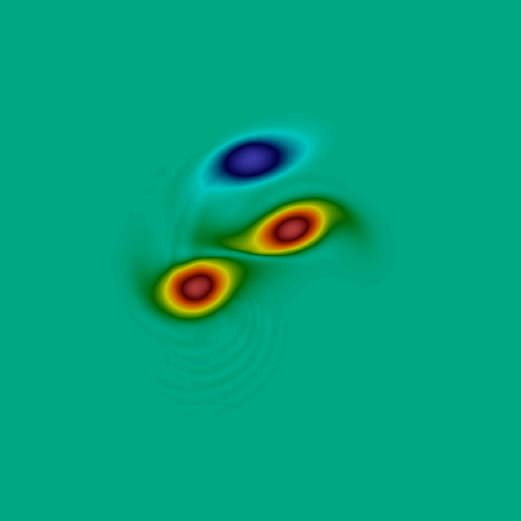
\includegraphics[scale=0.06]{data/Incompressible_Euler/Snapshots/red_17_2.png}\hspace{1em}
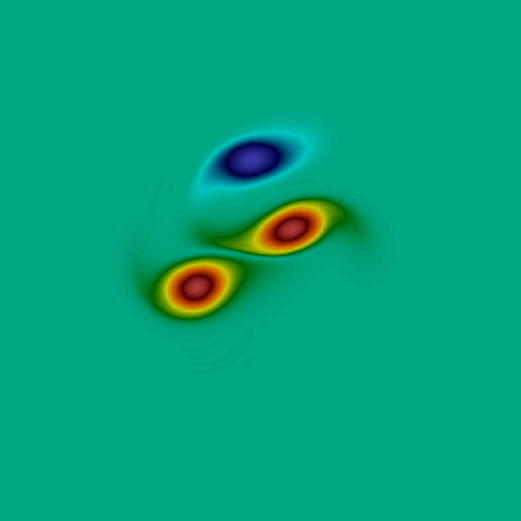
\includegraphics[scale=0.06]{data/Incompressible_Euler/Snapshots/red_35_2.png}\hspace{1em}
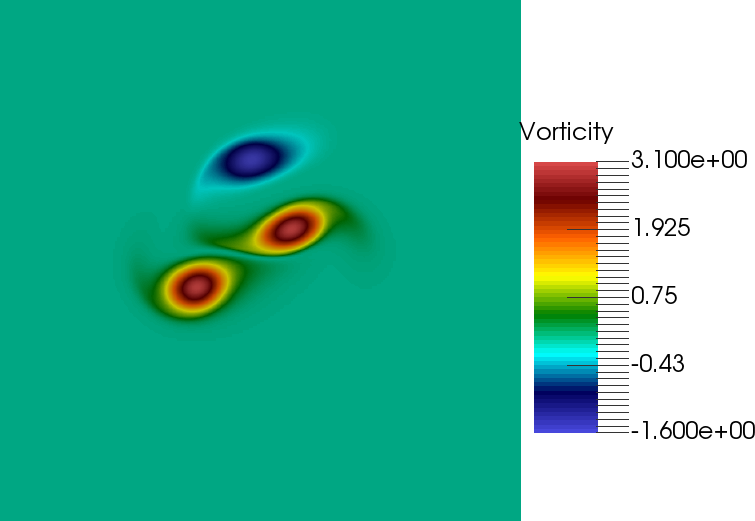
\includegraphics[scale=0.06]{data/Incompressible_Euler/Snapshots/Full_2.png}\\

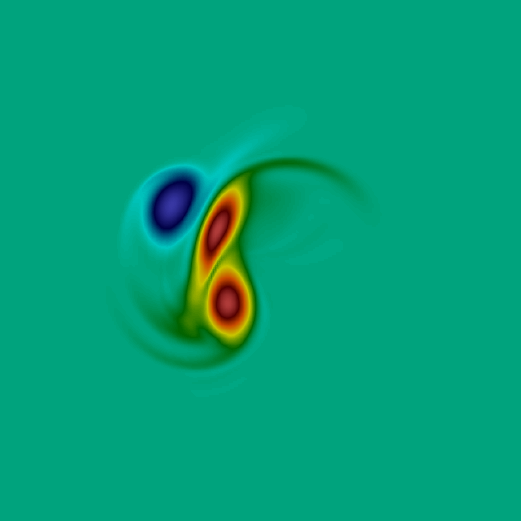
\includegraphics[scale=0.06]{data/Incompressible_Euler/Snapshots/red_17_3.png}\hspace{1em}
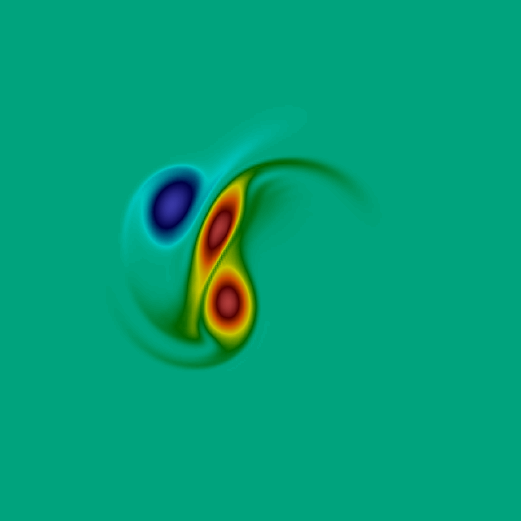
\includegraphics[scale=0.06]{data/Incompressible_Euler/Snapshots/red_35_3.png}\hspace{1em}
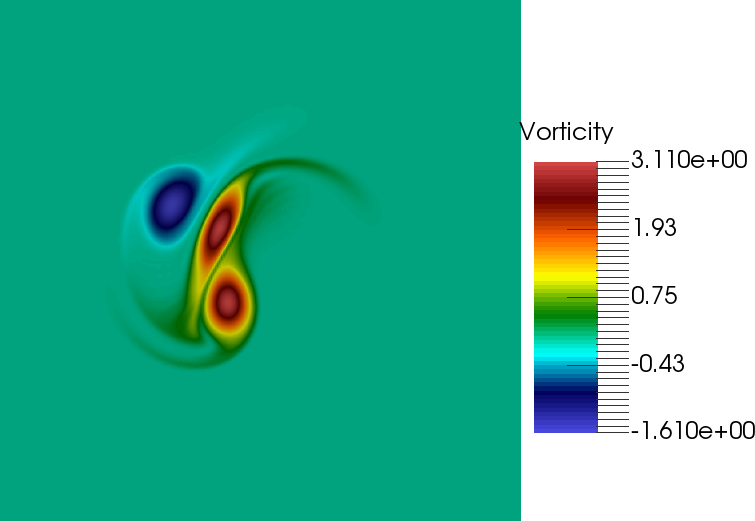
\includegraphics[scale=0.06]{data/Incompressible_Euler/Snapshots/Full_3.png}\\

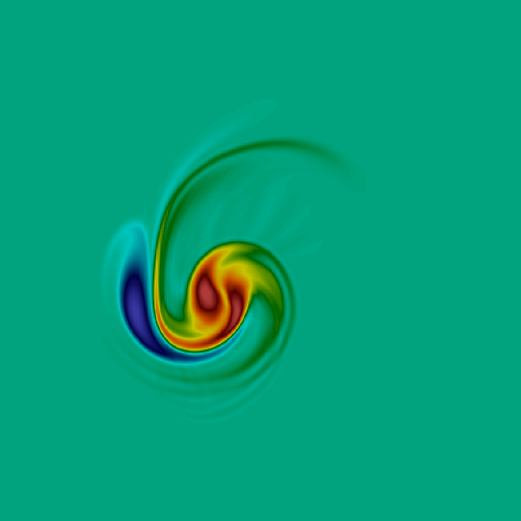
\includegraphics[scale=0.06]{data/Incompressible_Euler/Snapshots/red_17_4.png}\hspace{1em}
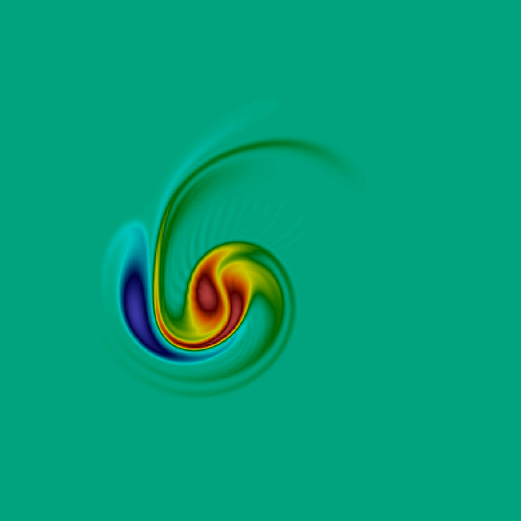
\includegraphics[scale=0.06]{data/Incompressible_Euler/Snapshots/red_35_4.png}\hspace{1em}
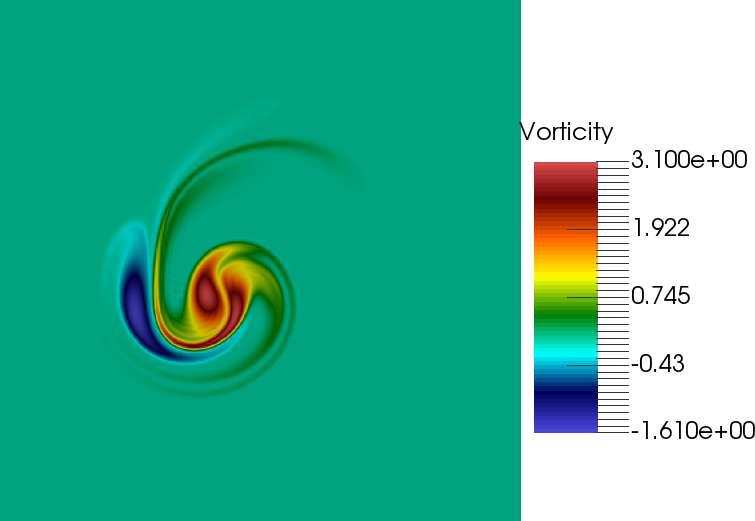
\includegraphics[scale=0.06]{data/Incompressible_Euler/Snapshots/Full_4.png}\\

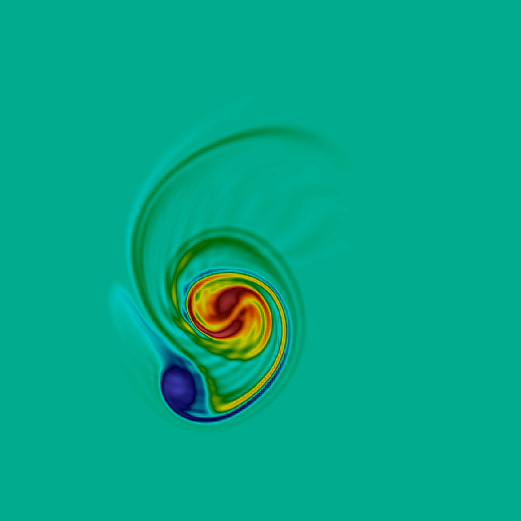
\includegraphics[scale=0.06]{data/Incompressible_Euler/Snapshots/red_17_5.png}\hspace{1em}
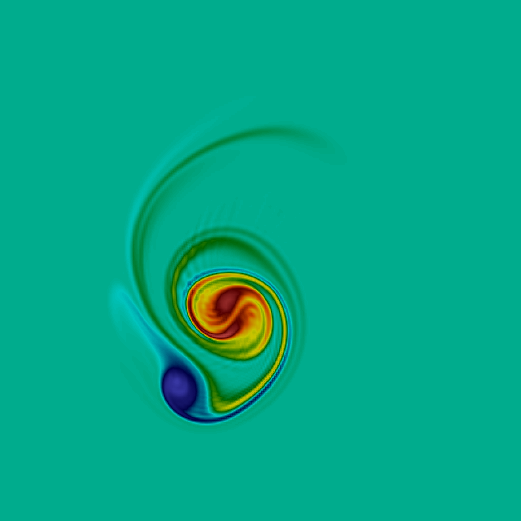
\includegraphics[scale=0.06]{data/Incompressible_Euler/Snapshots/red_35_5.png}\hspace{1em}
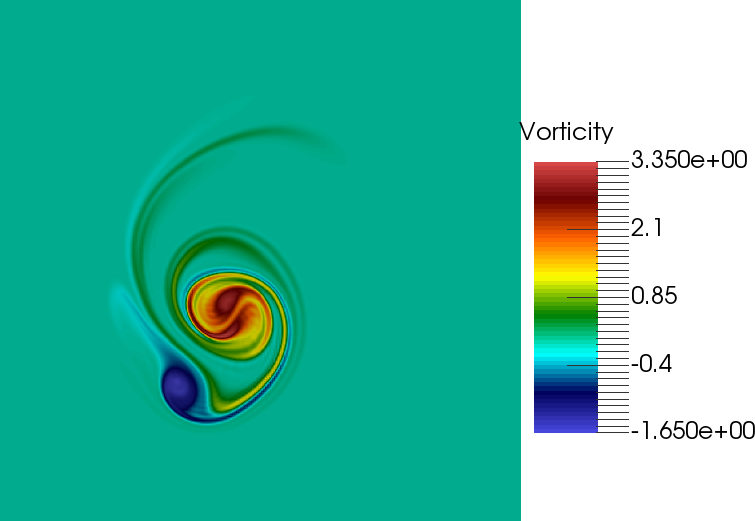
\includegraphics[scale=0.06]{data/Incompressible_Euler/Snapshots/Full_5.png}

\caption{Snapshots of the high-fidelity system and the reduced system at $t=\left\{ 4,8,12,18 \right\}$. From left to right: the snapshots of the reduced model with $k=17$, $k=35$ and the high fidelity solution.}
\label{fig:snap_solution_incompressible_Euler}
\end{figure}


%%%%%%%%%%%%%%%%%%%%%%%%%%%%%%%%%%%%%%%%%%
%%%%%%%%%% Singular values decay merging vorteces %%%%%%%%%%%
%%%%%%%%%%%%%%%%%%%%%%%%%%%%%%%%%%%%%%%%%%
\begin{figure}[t]
\centering
\begin{tikzpicture}[scale=0.5452]
    \begin{semilogyaxis}[ylabel = $\frac{\sigma_j}{\sum_i \sigma_i}$,
                 xlabel=Basis ,
                 label style={font=\large},
                 %legend pos=north east,
                 %legend entries={$k=24$ Div,$k=102$ Div,$k=201$ Div,$k=24$ Skew,$k=102$ Skew,$k=201$ Skew},
                 legend style={font=\large},
                 grid=both,
                 ticks=both,
                 width=0.7\linewidth, 
                 height=0.5\linewidth,
                 minor x tick num=1,
                 minor y tick num=2,	
                 yticklabel style={/pgf/number format/.cd,fixed,precision=9},
                 scaled x ticks = true,
                 enlargelimits=false,
                 scale only axis,
                 ymin=0,
                 ymax = 2,
                 samples = 100]
                 \addplot[color=black,style=solid,style=ultra thick]  table[x = x, y = s] {./data/Incompressible_Euler/Singular_values/sv.txt};
    \end{semilogyaxis}
\end{tikzpicture}
\caption{The decay of the singular values for the merging vortices problem. {\commnet \{please put this figure and figure 1 into a single figure (Left and right to each other)\} } }
\label{fig:RIC}
\end{figure}
\Cref{fig:approx_error_incompressible_Euler} shows the 2-norm error between the high-fidelity solution and the approximated solution. It is seen that the error decreases, consistently, as the number of basis vectors increase. Furthermore, the accuracy is maintained over the period of time integration.

The conservation of the kinetic energy is presented in \Cref{fig:energy_error_incompressible_Euler}. It is seen that even for a small number of basis vectors, where the solution is not well approximated, the kinetic energy is conserved. Furthermore, it is observed that the error in the kinetic energy, due to MOR, is constant in time. This helps with the robustness of the reduced system over long time-integration.


%%%%%%%%%%%%%%%%%%%%%%%%%%%%%%%%%%%%%%%%%%%
%%%%%%%%%% Approximation error and energy conservation %%%%%%%%%%
%%%%%%%%%%%%%%%%%%%%%%%%%%%%%%%%%%%%%%%%%%%
\begin{figure}[t]
\centering
\begin{subfigure}[]{0.47\linewidth}
\begin{tikzpicture}[scale=0.58]
    \begin{semilogyaxis}[ylabel = $\left | \mathbf{v}(t)-\mathbf{v}^r(t) \right |^2$,
                 xlabel=$t$,
                 label style={font=\large},
                 legend style={font=\large},
                 grid=both,
                 ticks=both,
                 width=1.4\linewidth, 
                 height=1.0\linewidth,
                 minor x tick num=1,
                 minor y tick num=2,	
                 yticklabel style={/pgf/number format/.cd,fixed,precision=9},
                 scaled x ticks = true,
                 enlargelimits=false,
                 scale only axis,
                 samples = 100,
                 cycle list name=exotic]
                 \addplot+[style=solid,style=ultra thick]  table[x = time, y = error] {./data/Incompressible_Euler/Approximation_Error/err_5.txt};
                 \addplot+[style=solid,style=ultra thick]  table[x = time, y = error] {./data/Incompressible_Euler/Approximation_Error/err_8.txt};
                 \addplot+[style=solid,style=ultra thick]  table[x = time, y = error] {./data/Incompressible_Euler/Approximation_Error/err_11.txt};
                 \addplot+[style=solid,style=ultra thick]  table[x = time, y = error] {./data/Incompressible_Euler/Approximation_Error/err_14.txt};
                 \addplot+[style=solid,style=ultra thick]  table[x = time, y = error] {./data/Incompressible_Euler/Approximation_Error/err_23.txt};
                 \addplot+[style=solid,style=ultra thick]  table[x = time, y = error] {./data/Incompressible_Euler/Approximation_Error/err_26.txt};
                 \addplot+[style=solid,style=ultra thick]  table[x = time, y = error] {./data/Incompressible_Euler/Approximation_Error/err_29.txt};
                 \addplot+[style=solid,style=ultra thick]  table[x = time, y = error] {./data/Incompressible_Euler/Approximation_Error/err_35.txt};
    \end{semilogyaxis}
\end{tikzpicture}
\caption{}
\label{fig:approx_error_incompressible_Euler}
\end{subfigure} \hfill
\begin{subfigure}[]{0.47\linewidth}
\begin{tikzpicture}[scale=0.58]
    \begin{axis}[ylabel = $|K(t)-K_r^{r}(t)|$,
                 xlabel=$t$,
                 label style={font=\large},
                 legend pos=south west,
                 legend entries={$k=5$ , $k=8$, $k=11$, $k=14$, $k=23$, $k=26$, $k=29$, $k=35$},
                 legend style={font=\large},
                 grid=both,
                 ticks=both,
                 width=1.4\linewidth, 
                 height=1.0\linewidth,
                 minor x tick num=1,
                 minor y tick num=2,	
                 yticklabel style={/pgf/number format/.cd,fixed,precision=9},
                 scaled x ticks = true,
                 enlargelimits=false,
                 scale only axis,
                 ymax = 0.5598,
                 samples = 100,
                 cycle list name=exotic]
                 \addplot+[style=solid,style=ultra thick]  table[x = time, y = error] {./data/Incompressible_Euler/Energy_conservation/ene_full_5.txt};
                 \addplot+[style=solid,style=ultra thick]  table[x = time, y = error] {./data/Incompressible_Euler/Energy_conservation/ene_full_8.txt};
                 \addplot+[style=solid,style=ultra thick]  table[x = time, y = error] {./data/Incompressible_Euler/Energy_conservation/ene_full_11.txt};
                 \addplot+[style=solid,style=ultra thick]  table[x = time, y = error] {./data/Incompressible_Euler/Energy_conservation/ene_full_14.txt};
                 \addplot+[style=solid,style=ultra thick]  table[x = time, y = error] {./data/Incompressible_Euler/Energy_conservation/ene_full_23.txt};
                 \addplot+[style=solid,style=ultra thick]  table[x = time, y = error] {./data/Incompressible_Euler/Energy_conservation/ene_full_26.txt};
                 \addplot+[style=solid,style=ultra thick]  table[x = time, y = error] {./data/Incompressible_Euler/Energy_conservation/ene_full_29.txt};
                 \addplot+[style=solid,style=ultra thick]  table[x = time, y = error] {./data/Incompressible_Euler/Energy_conservation/ene_full_35.txt};
    \end{axis}
\end{tikzpicture}
\caption{}
\label{fig:energy_error_incompressible_Euler}
\end{subfigure}
\label{fig:energy_approx_err}
\caption{(\protect\subref{fig:approx_error_incompressible_Euler}) Evolution of 2-norm error in velocity, between the high-fidelity system and the reduced system. (\protect\subref{fig:energy_error_incompressible_Euler}) Conservation of the kinetic energy. {\commnet \{ in fig a $y$ axis: $\| u - \tilde u \|_2$ \} \{ in fig b $|k - \tilde K|$ \}}  }
\end{figure}


\subsection{The Compressible Euler Equation}
\subsubsection{2D Kelvin-Helmholtz instability}
%%%%%%%%%%%%%%%%%%%%%%%%%%%%%%%%%%%%%%%%%
%%%%%%%%%%%%% Singular values KH problem %%%%%%%%%%%%%%
%%%%%%%%%%%%%%%%%%%%%%%%%%%%%%%%%%%%%%%%%

\subsubsection{1D Shock problem}
%%%%%%%%%%%%%%%%%%%%%%%%%%%%%%%%%%%%%%%%%
%%%%%%%%%%%%% Singular values 1D problem %%%%%%%%%%%%%%
%%%%%%%%%%%%%%%%%%%%%%%%%%%%%%%%%%%%%%%%%
\begin{figure}
\centering
\begin{tikzpicture}[scale=0.5452]
    \begin{semilogyaxis}[ylabel = $\frac{\sigma_j}{\sum_i \sigma_i}$,
                 xlabel=Basis,
                 label style={font=\large},
                 legend style={font=\large},
                 grid=both,
                 ticks=both,
                 width=0.7\linewidth, 
                 height=0.5\linewidth,
                 minor x tick num=1,
                 minor y tick num=2,	
                 yticklabel style={/pgf/number format/.cd,fixed,precision=9},
                 scaled x ticks = true,
                 enlargelimits=false,
                 scale only axis,
                 ymin=0,
                 ymax = 2,
                 samples = 100]
                 \addplot[color=black,style=solid,style=ultra thick]  table[x = n, y = sing_values] {./data/Compressible_Euler/1D/Singular_values/sv.txt};
    \end{semilogyaxis}
\end{tikzpicture}
\caption{Singular values decay of the snapshot matrix related to POD algorithms for the 1D compressible Euler problem.}
\end{figure}

%%%%%%%%%%%%%%%%%%%%%%%%%%%%%%%%%%%%%%%%%%%%
%%%%%%%%%%%%% Mass, Total momentum & Energy %%%%%%%%%%%%%%
%%%%%%%%%%%%%%%%%%%%%%%%%%%%%%%%%%%%%%%%%%%%
\begin{figure}
  \centering
  % MASS
  \begin{subfigure}[]{0.48\linewidth}
  \begin{tikzpicture}[scale=0.55]
    \begin{axis}[ylabel = Mass,
                 xlabel=$t$,
                 label style={font=\large},
                 legend pos=north east,
                 legend entries={$k=102$ Conv,$k=201$ Conv,$k=102$ Div,$k=201$ Div,$k=102$ Skew,$k=201$ Skew},
                 legend style={font=\large},
                 grid=both,
                 ticks=both,
                 width=1.4\linewidth, 
                 height=1.0\linewidth,
                 minor x tick num=1,
                 minor y tick num=2,	
                 yticklabel style={/pgf/number format/.cd,fixed,precision=9},
                 scaled x ticks = true,
                 enlargelimits=false,
                 scale only axis,
                 ymin=0,
                 ymax = 2,
                 samples = 100]
                 \addplot[color=red,style=dashdotted,style=ultra thick]  table[x = time, y = quantity] {./data/Compressible_Euler/1D/convective_data/mass_102_1.txt};
                 \addplot[color=blue,style=dashdotted,style=ultra thick]  table[x = time, y = quantity] {./data/Compressible_Euler/1D/convective_data/mass_201_1.txt};
                 \addplot[color=red,style=dashed,style=ultra thick]  table[x = time, y = quantity] {./data/Compressible_Euler/1D/divergence_data/mass_102_1.txt};
                 \addplot[color=blue,style=dashed,style=ultra thick]  table[x = time, y = quantity] {./data/Compressible_Euler/1D/divergence_data/mass_201_1.txt};
                 \addplot[color=red,style=solid,style=ultra thick]  table[x = time, y = quantity] {./data/Compressible_Euler/1D/skew_symm_data/mass_102_1.txt};
                 \addplot[color=blue,style=solid,style=ultra thick]  table[x = time, y = quantity] {./data/Compressible_Euler/1D/skew_symm_data/mass_201_1.txt};
    \end{axis}%  
  \end{tikzpicture}
  \end{subfigure}\hfill% 
  % MASS (focus)
  \begin{subfigure}[]{0.48\linewidth}
  \begin{tikzpicture}[scale=0.55]
    \begin{axis}[xlabel=$t$,
                 label style={font=\large},
                 legend pos=south west,
                 legend entries={$k=24$ Skew,$k=102$ Skew,$k=201$ Skew},
                 legend style={font=\large},
                 grid=both,
                 ticks=both,
                 width=1.4\linewidth, 
                 height=1.0\linewidth,
                 minor x tick num=1,
                 minor y tick num=2,	
                 yticklabel style={/pgf/number format/.cd,fixed,precision=9},
                 scaled x ticks = true,
                 enlargelimits=false,
                 scale only axis,
                 ymax=0.5000001]
                 \addplot[color=black!50!green,style=solid,style=ultra thick]  table[x = time, y = quantity] {./data/Compressible_Euler/1D/skew_symm_data/mass_24_1.txt};
                 \addplot[color=red,style=solid,style=ultra thick]  table[x = time, y = quantity] {./data/Compressible_Euler/1D/skew_symm_data/mass_102_1.txt};
                 \addplot[color=blue,style=solid,style=ultra thick]  table[x = time, y = quantity] {./data/Compressible_Euler/1D/skew_symm_data/mass_201_1.txt};
    \end{axis}%  
  \end{tikzpicture}
  \end{subfigure}
 % TOTAL MOMENTUM
  \begin{subfigure}[]{0.48\linewidth}
  \begin{tikzpicture}[scale=0.55]
    \begin{axis}[ylabel = Momentum,
                 xlabel=$t$,
                 label style={font=\large},
                 legend pos=north east,
                 %legend entries={$k=24$ Div,$k=102$ Div,$k=201$ Div,$k=24$ Skew,$k=102$ Skew,$k=201$ Skew},
                 legend style={font=\large},
                 grid=both,
                 ticks=both,
                 width=1.4\linewidth, 
                 height=1.0\linewidth,
                 minor x tick num=1,
                 minor y tick num=2,	
                 yticklabel style={/pgf/number format/.cd,fixed,precision=9},
                 scaled x ticks = true,
                 enlargelimits=false,
                 scale only axis,
                 ymin=1,
                 ymax = 2,
                 samples = 100]
                 \addplot[color=red,style=dashdotted,style=ultra thick]  table[x = time, y = quantity] {./data/Compressible_Euler/1D/convective_data/momentum_102_1.txt};
                 \addplot[color=blue,style=dashdotted,style=ultra thick]  table[x = time, y = quantity] {./data/Compressible_Euler/1D/convective_data/momentum_201_1.txt};
                 \addplot[color=red,style=dashed,style=ultra thick]  table[x = time, y = quantity] {./data/Compressible_Euler/1D/divergence_data/momentum_102_1.txt};
                 \addplot[color=blue,style=dashed,style=ultra thick]  table[x = time, y = quantity] {./data/Compressible_Euler/1D/divergence_data/momentum_201_1.txt};
                 \addplot[color=red,style=solid,style=ultra thick]  table[x = time, y = quantity] {./data/Compressible_Euler/1D/skew_symm_data/momentum_102_1.txt};
                 \addplot[color=blue,style=solid,style=ultra thick]  table[x = time, y = quantity] {./data/Compressible_Euler/1D/skew_symm_data/momentum_201_1.txt};
    \end{axis}%  
  \end{tikzpicture} 
  \end{subfigure}\hfill% 
 % TOTAL MOMENTUM (focus)
  \begin{subfigure}[]{0.48\linewidth}
  \begin{tikzpicture}[scale=0.55]
    \begin{axis}[xlabel=$t$,
                 label style={font=\large},
                 legend pos=south west,
                 legend style={font=\large},
                 grid=both,
                 ticks=both,
                 width=1.4\linewidth, 
                 height=1.0\linewidth,
                 minor x tick num=1,
                 minor y tick num=2,	
                 yticklabel style={/pgf/number format/.cd,fixed,precision=9},
                 scaled x ticks = true,
                 enlargelimits=false,
                 ymax=1.04963,
                 scale only axis]
                 \addplot[color=black!50!green,style=solid,style=ultra thick]  table[x = time, y = quantity] {./data/Compressible_Euler/1D/skew_symm_data/momentum_24_1.txt};
                 \addplot[color=red,style=solid,style=ultra thick]  table[x = time, y = quantity] {./data/Compressible_Euler/1D/skew_symm_data/momentum_102_1.txt};
                 \addplot[color=blue,style=solid,style=ultra thick]  table[x = time, y = quantity] {./data/Compressible_Euler/1D/skew_symm_data/momentum_201_1.txt};
    \end{axis}%  
  \end{tikzpicture}
  \end{subfigure}
 % ENERGY
  \begin{subfigure}[]{0.48\linewidth}
  \begin{tikzpicture}[scale=0.55]
    \begin{axis}[ylabel = Energy,
                 xlabel=$t$,
                 label style={font=\large},
                 legend pos=north east,
                 %legend entries={$k=24$ Div,$k=102$ Div,$k=201$ Div,$k=24$ Skew,$k=102$ Skew,$k=201$ Skew},
                 legend style={font=\large},
                 grid=both,
                 ticks=both,
                 width=1.4\linewidth, 
                 height=1.0\linewidth,
                 minor x tick num=1,
                 minor y tick num=2,	
                 yticklabel style={/pgf/number format/.cd,fixed,precision=9},
                 scaled x ticks = true,
                 enlargelimits=false,
                 scale only axis,
                 ymin=2.5,
                 ymax = 4.5,
                 samples = 100]
                 \addplot[color=red,style=dashed,style=ultra thick]  table[x = time, y = quantity] {./data/Compressible_Euler/1D/convective_data/energy_102_1.txt};
                 \addplot[color=blue,style=dashed,style=ultra thick]  table[x = time, y = quantity] {./data/Compressible_Euler/1D/convective_data/energy_201_1.txt};                
                 \addplot[color=red,style=dashed,style=ultra thick]  table[x = time, y = quantity] {./data/Compressible_Euler/1D/divergence_data/energy_102_1.txt};
                 \addplot[color=blue,style=dashed,style=ultra thick]  table[x = time, y = quantity] {./data/Compressible_Euler/1D/divergence_data/energy_201_1.txt};
                 \addplot[color=red,style=solid,style=ultra thick]  table[x = time, y = quantity] {./data/Compressible_Euler/1D/skew_symm_data/energy_102_1.txt};
                 \addplot[color=blue,style=solid,style=ultra thick]  table[x = time, y = quantity] {./data/Compressible_Euler/1D/skew_symm_data/energy_201_1.txt};
    \end{axis}%  
  \end{tikzpicture} 
  \caption{}
  \label{conservation_1D}
  \end{subfigure}\hfill% 
 % ENERGY (focus)
  \begin{subfigure}[]{0.48\linewidth}
  \begin{tikzpicture}[scale=0.55]
    \begin{axis}[xlabel=$t$,
                 label style={font=\large},
                 legend pos=south west,
                 legend style={font=\large},
                 grid=both,
                 ticks=both,
                 width=1.4\linewidth, 
                 height=1.0\linewidth,
                 minor x tick num=1,
                 minor y tick num=2,	
                 yticklabel style={/pgf/number format/.cd,fixed,precision=9},
                 scaled x ticks = true,
                 enlargelimits=false,
                 scale only axis,
                 ymax = 2.87438]
                 \addplot[color=black!50!green,style=solid,style=ultra thick]  table[x = time, y = quantity] {./data/Compressible_Euler/1D/skew_symm_data/energy_24_1.txt};
                 \addplot[color=red,style=solid,style=ultra thick]  table[x = time, y = quantity] {./data/Compressible_Euler/1D/skew_symm_data/energy_102_1.txt};
                 \addplot[color=blue,style=solid,style=ultra thick]  table[x = time, y = quantity] {./data/Compressible_Euler/1D/skew_symm_data/energy_201_1.txt};
    \end{axis}%  
  \end{tikzpicture}
  \caption{}
  \label{conservation_1D_focus}
  \end{subfigure}
  \caption{(\protect\subref{conservation_1D})  Evolution of the three conserved quantities for the reduced solution of the compressible Euler equation (mass, total momentum and total energy).  The divergent, advective and skew-symmetric formulations have been considered and $k=102,204$ basis are used for the reduction. (\protect\subref{conservation_1D_focus}) Focus on the conserved quantity in case of stable reduction using the skew-symmetric formulation.} 
\end{figure}

%%%%%%%%%%%%%%%%%%%%%%%%%%%%%%%%%%%%%%%%%%%%
%%%%%%%%%%%%%%%% Approximation Error %%%%%%%%%%%%%%%%%
%%%%%%%%%%%%%%%%%%%%%%%%%%%%%%%%%%%%%%%%%%%%
\begin{figure}
\centering
\begin{subfigure}[]{0.48\linewidth}
  \begin{tikzpicture}[scale=0.55]
    \begin{semilogyaxis}[xlabel=$t$,
                 ylabel=$e(t)$
                 label style={font=\large},
                 legend pos=outer north east,
                 legend style={font=\large},
                 legend entries={$k=75$,$k=126$,$k=177$,$k=225$,$k=276$,$k=327$,$k=375$,$k=426$},
                 grid=both,
                 ticks=both,
                 width=1.4\linewidth, 
                 height=1.0\linewidth,
                 minor x tick num=1,
                 minor y tick num=2,	
                 yticklabel style={/pgf/number format/.cd,fixed,precision=9},
                 scaled x ticks = true,
                 enlargelimits=false,
                 scale only axis,
                 cycle list name=exotic]
                 \addplot+[style=solid,style=ultra thick]  table[x = time, y = quantity] {./data/Compressible_Euler/1D/error/error_75.txt};  
                 \addplot+[style=solid,style=ultra thick]  table[x = time, y = quantity] {./data/Compressible_Euler/1D/error/error_126.txt};      
                 \addplot+[style=solid,style=ultra thick]  table[x = time, y = quantity] {./data/Compressible_Euler/1D/error/error_177.txt}; 
                 \addplot+[style=solid,style=ultra thick]  table[x = time, y = quantity] {./data/Compressible_Euler/1D/error/error_225.txt};      
                 \addplot+[style=solid,style=ultra thick]  table[x = time, y = quantity] {./data/Compressible_Euler/1D/error/error_276.txt};  
                 \addplot+[style=solid,style=ultra thick]  table[x = time, y = quantity] {./data/Compressible_Euler/1D/error/error_327.txt}; 
                 \addplot+[style=solid,style=ultra thick]  table[x = time, y = quantity] {./data/Compressible_Euler/1D/error/error_375.txt};      
                 \addplot+[style=solid,style=ultra thick]  table[x = time, y = quantity] {./data/Compressible_Euler/1D/error/error_426.txt};              
    \end{semilogyaxis}%  
  \end{tikzpicture}
\end{subfigure}
\caption{Evolution in time of the error  between the high fidelity solution of the 1D compressible Euler and the reduced solution for different number of basis $k$. As error measure we consider $e(t)=\sqrt{\|\mathbf{r}-\mathbf{r}^r\|^2+\|\mathbf{ur}-\mathbf{ur}^r\|^2\|\mathbf{p}-\mathbf{p}^r\|^2}$}.
\end{figure}

%%%%%%%%%%%%%%%%%%%%%%%%%%%%%%%%%%%%%%%%%%%%
%%%%%%%%%%%%% Snapshot of pressure and density %%%%%%%%%%%%%%
%%%%%%%%%%%%%%%%%%%%%%%%%%%%%%%%%%%%%%%%%%%%
\begin{figure}
\centering
\begin{subfigure}[]{0.47\linewidth}
\begin{tikzpicture}[scale=0.58]
    \begin{axis}[xlabel=$x$,
                 ylabel=Density,
                 label style={font=\large},
                 legend pos=south west,
                 legend entries={HF,$k=24$ Div,$k=102$ Div,$k=201$ Div,$k=24$ Skew,$k=102$ Skew,$k=201$ Skew},
                 legend style={font=\large},
                 grid=both,
                 ticks=both,
                 width=1.4\linewidth, 
                 height=1.0\linewidth,
                 minor x tick num=1,
                 minor y tick num=2,	
                 yticklabel style={/pgf/number format/.cd,fixed,precision=9},
                 scaled x ticks = true,
                 enlargelimits=false,
                 scale only axis]
                 \addplot[color=black,style=solid,style=ultra thick]  table[x = time, y = energy] {./data/Compressible_Euler/1D/Snapshots/density_exact_300.txt};
                 \addplot[color=red,style=dashed,style=ultra thick]  table[x = time, y = energy] {./data/Compressible_Euler/1D/Snapshots/density_approx_unstable_24_300.txt};
                 \addplot[color=blue,style=dashed,style=ultra thick]  table[x = time, y = energy] {./data/Compressible_Euler/1D/Snapshots/density_approx_unstable_102_300.txt};
                 \addplot[color=black!50!green,style=dashed,style=ultra thick]  table[x = time, y = energy] {./data/Compressible_Euler/1D/Snapshots/density_approx_unstable_201_300.txt};
                 \addplot[color=red,style=solid,style=ultra thick]  table[x = time, y = energy] {./data/Compressible_Euler/1D/Snapshots/density_approx_24_300.txt};
                 \addplot[color=blue,style=solid,style=ultra thick]  table[x = time, y = energy] {./data/Compressible_Euler/1D/Snapshots/density_approx_102_300.txt};
                 \addplot[color=black!50!green,style=solid,style=ultra thick]  table[x = time, y = energy] {./data/Compressible_Euler/1D/Snapshots/density_approx_201_300.txt};
    \end{axis}% 
\end{tikzpicture}
\end{subfigure} 
\begin{subfigure}[]{0.47\linewidth}
\begin{tikzpicture}[scale=0.58]
    \begin{axis}[xlabel=$x$,
                 ylabel=Pressure,
                 label style={font=\large},
                 legend pos=south west,
                 %legend entries={HF,$k=24$ Div,$k=102$ Div,$k=201$ Div,$k=24$ Skew,$k=102$ Skew,$k=201$ Skew},
                 legend style={font=\large},
                 grid=both,
                 ticks=both,
                 width=1.4\linewidth, 
                 height=1.0\linewidth,
                 minor x tick num=1,
                 minor y tick num=2,	
                 yticklabel style={/pgf/number format/.cd,fixed,precision=9},
                 scaled x ticks = true,
                 enlargelimits=false,
                 scale only axis]
                 \addplot[color=black,style=solid,style=ultra thick]  table[x = time, y = energy] {./data/Compressible_Euler/1D/Snapshots/pressure_exact_300.txt};
                 \addplot[color=red,style=dashed,style=ultra thick]  table[x = time, y = energy] {./data/Compressible_Euler/1D/Snapshots/pressure_approx_unstable_24_300.txt};
                 \addplot[color=blue,style=dashed,style=ultra thick]  table[x = time, y = energy] {./data/Compressible_Euler/1D/Snapshots/pressure_approx_unstable_102_300.txt};
                 \addplot[color=black!50!green,style=dashed,style=ultra thick]  table[x = time, y = energy] {./data/Compressible_Euler/1D/Snapshots/pressure_approx_unstable_201_300.txt};
                 \addplot[color=red,style=solid,style=ultra thick]  table[x = time, y = energy] {./data/Compressible_Euler/1D/Snapshots/pressure_approx_24_300.txt};
                 \addplot[color=blue,style=solid,style=ultra thick]  table[x = time, y = energy] {./data/Compressible_Euler/1D/Snapshots/pressure_approx_102_300.txt};
                 \addplot[color=black!50!green,style=solid,style=ultra thick]  table[x = time, y = energy] {./data/Compressible_Euler/1D/Snapshots/pressure_approx_201_300.txt};
    \end{axis}% 
\end{tikzpicture}
\label{density_reduction}
\end{subfigure}

\begin{subfigure}[]{0.47\linewidth}
\begin{tikzpicture}[scale=0.58]
    \begin{axis}[xlabel=$x$,
                 ylabel=Density,
                 label style={font=\large},
                 legend pos=south west,
                 legend entries={HF,$k=24$ Div,$k=102$ Div,$k=201$ Div,$k=24$ Skew,$k=102$ Skew,$k=201$ Skew},
                 legend style={font=\large},
                 grid=both,
                 ticks=both,
                 width=1.4\linewidth, 
                 height=1.0\linewidth,
                 minor x tick num=1,
                 minor y tick num=2,	
                 yticklabel style={/pgf/number format/.cd,fixed,precision=9},
                 scaled x ticks = true,
                 enlargelimits=false,
                 scale only axis]
                 \addplot[color=black,style=solid,style=ultra thick]  table[x = time, y = energy] {./data/Compressible_Euler/1D/Snapshots/density_exact_1000.txt};
                 \addplot[color=red,style=dashed,style=ultra thick]  table[x = time, y = energy] {./data/Compressible_Euler/1D/Snapshots/density_approx_unstable_24_1000.txt};
                 \addplot[color=blue,style=dashed,style=ultra thick]  table[x = time, y = energy] {./data/Compressible_Euler/1D/Snapshots/density_approx_unstable_102_1000.txt};
                 \addplot[color=black!50!green,style=dashed,style=ultra thick]  table[x = time, y = energy] {./data/Compressible_Euler/1D/Snapshots/density_approx_unstable_201_1000.txt};
                 \addplot[color=red,style=solid,style=ultra thick]  table[x = time, y = energy] {./data/Compressible_Euler/1D/Snapshots/density_approx_24_1000.txt};
                 \addplot[color=blue,style=solid,style=ultra thick]  table[x = time, y = energy] {./data/Compressible_Euler/1D/Snapshots/density_approx_102_1000.txt};
                 \addplot[color=black!50!green,style=solid,style=ultra thick]  table[x = time, y = energy] {./data/Compressible_Euler/1D/Snapshots/density_approx_201_1000.txt};
    \end{axis}% 
\end{tikzpicture}
\end{subfigure} 
\begin{subfigure}[]{0.47\linewidth}
\begin{tikzpicture}[scale=0.58]
    \begin{axis}[xlabel=$x$,
                 ylabel=Pressure,
                 label style={font=\large},
                 legend pos=south west,
                 %legend entries={HF,$k=24$ Div,$k=102$ Div,$k=201$ Div,$k=24$ Skew,$k=102$ Skew,$k=201$ Skew},
                 legend style={font=\large},
                 grid=both,
                 ticks=both,
                 width=1.4\linewidth, 
                 height=1.0\linewidth,
                 minor x tick num=1,
                 minor y tick num=2,	
                 yticklabel style={/pgf/number format/.cd,fixed,precision=9},
                 scaled x ticks = true,
                 enlargelimits=false,
                 scale only axis]
                 \addplot[color=black,style=solid,style=ultra thick]  table[x = time, y = energy] {./data/Compressible_Euler/1D/Snapshots/pressure_exact_1000.txt};
                 \addplot[color=red,style=dashed,style=ultra thick]  table[x = time, y = energy] {./data/Compressible_Euler/1D/Snapshots/pressure_approx_unstable_24_1000.txt};
                 \addplot[color=blue,style=dashed,style=ultra thick]  table[x = time, y = energy] {./data/Compressible_Euler/1D/Snapshots/pressure_approx_unstable_102_1000.txt};
                 \addplot[color=black!50!green,style=dashed,style=ultra thick]  table[x = time, y = energy] {./data/Compressible_Euler/1D/Snapshots/pressure_approx_unstable_201_1000.txt};
                 \addplot[color=red,style=solid,style=ultra thick]  table[x = time, y = energy] {./data/Compressible_Euler/1D/Snapshots/pressure_approx_24_1000.txt};
                 \addplot[color=blue,style=solid,style=ultra thick]  table[x = time, y = energy] {./data/Compressible_Euler/1D/Snapshots/pressure_approx_102_1000.txt};
                 \addplot[color=black!50!green,style=solid,style=ultra thick]  table[x = time, y = energy] {./data/Compressible_Euler/1D/Snapshots/pressure_approx_201_1000.txt};
    \end{axis}% 
\end{tikzpicture}
\end{subfigure}

\begin{subfigure}[]{0.47\linewidth}
\begin{tikzpicture}[scale=0.58]
    \begin{axis}[xlabel=$x$,
                 ylabel=Density,
                 label style={font=\large},
                 legend pos=south west,
                 legend entries={HF,$k=24$ Div,$k=102$ Div,$k=201$ Div,$k=24$ Skew,$k=102$ Skew,$k=201$ Skew},
                 legend style={font=\large},
                 grid=both,
                 ticks=both,
                 width=1.4\linewidth, 
                 height=1.0\linewidth,
                 minor x tick num=1,
                 minor y tick num=2,	
                 yticklabel style={/pgf/number format/.cd,fixed,precision=9},
                 scaled x ticks = true,
                 enlargelimits=false,
                 scale only axis]
                 \addplot[color=black,style=solid,style=ultra thick]  table[x = time, y = energy] {./data/Compressible_Euler/1D/Snapshots/density_exact_3000.txt};
                 \addplot[color=red,style=dashed,style=ultra thick]  table[x = time, y = energy] {./data/Compressible_Euler/1D/Snapshots/density_approx_unstable_24_3000.txt};
                 \addplot[color=blue,style=dashed,style=ultra thick]  table[x = time, y = energy] {./data/Compressible_Euler/1D/Snapshots/density_approx_unstable_102_3000.txt};
                 \addplot[color=black!50!green,style=dashed,style=ultra thick]  table[x = time, y = energy] {./data/Compressible_Euler/1D/Snapshots/density_approx_unstable_201_3000.txt};
                 \addplot[color=red,style=solid,style=ultra thick]  table[x = time, y = energy] {./data/Compressible_Euler/1D/Snapshots/density_approx_24_3000.txt};
                 \addplot[color=blue,style=solid,style=ultra thick]  table[x = time, y = energy] {./data/Compressible_Euler/1D/Snapshots/density_approx_102_3000.txt};
                 \addplot[color=black!50!green,style=solid,style=ultra thick]  table[x = time, y = energy] {./data/Compressible_Euler/1D/Snapshots/density_approx_201_3000.txt};
    \end{axis}% 
\end{tikzpicture}
\caption{}
\label{density_reduction_1D}
\end{subfigure} 
\begin{subfigure}[]{0.47\linewidth}
\begin{tikzpicture}[scale=0.58]
    \begin{axis}[xlabel=$x$,
                 ylabel=Pressure,
                 label style={font=\large},
                 legend pos=south west,
                 %legend entries={HF,$k=24$ Div,$k=102$ Div,$k=201$ Div,$k=24$ Skew,$k=102$ Skew,$k=201$ Skew},
                 legend style={font=\large},
                 grid=both,
                 ticks=both,
                 width=1.4\linewidth, 
                 height=1.0\linewidth,
                 minor x tick num=1,
                 minor y tick num=2,	
                 yticklabel style={/pgf/number format/.cd,fixed,precision=9},
                 scaled x ticks = true,
                 enlargelimits=false,
                 scale only axis]
                 \addplot[color=black,style=solid,style=ultra thick]  table[x = time, y = energy] {./data/Compressible_Euler/1D/Snapshots/pressure_exact_3000.txt};
                 \addplot[color=red,style=dashed,style=ultra thick]  table[x = time, y = energy] {./data/Compressible_Euler/1D/Snapshots/pressure_approx_unstable_24_3000.txt};
                 \addplot[color=blue,style=dashed,style=ultra thick]  table[x = time, y = energy] {./data/Compressible_Euler/1D/Snapshots/pressure_approx_unstable_102_3000.txt};
                 \addplot[color=black!50!green,style=dashed,style=ultra thick]  table[x = time, y = energy] {./data/Compressible_Euler/1D/Snapshots/pressure_approx_unstable_201_3000.txt};
                 \addplot[color=red,style=solid,style=ultra thick]  table[x = time, y = energy] {./data/Compressible_Euler/1D/Snapshots/pressure_approx_24_3000.txt};
                 \addplot[color=blue,style=solid,style=ultra thick]  table[x = time, y = energy] {./data/Compressible_Euler/1D/Snapshots/pressure_approx_102_3000.txt};
                 \addplot[color=black!50!green,style=solid,style=ultra thick]  table[x = time, y = energy] {./data/Compressible_Euler/1D/Snapshots/pressure_approx_201_3000.txt};
    \end{axis}% 
\end{tikzpicture}
\caption{}
\label{pressure_reduction_1D}
\end{subfigure}
\caption{Qualitative comparison between different formulations for the reduced model in terms of density (\protect\subref{density_reduction_1D})  and pressure(\protect\subref{pressure_reduction_1D}) at $t=0.1,0.3$ and $1$s. Results for the advective formulation are not showed here because the related reduced solutions are unstable after few time steps.}
\end{figure}

\begin{figure}[h!]
\centering
\begin{subfigure}[]{0.47\linewidth}
\begin{tikzpicture}[scale=0.58]
    \begin{axis}[ylabel = e(T),
                 xlabel=Basis DEIM,
                 label style={font=\large},
                 legend pos=north east,
                 legend entries={POD+DEIM,POD},
                 legend style={font=\large},
                 grid=both,
                 ticks=both,
                 width=1.4\linewidth, 
                 height=1\linewidth,
                 minor x tick num=1,
                 minor y tick num=2,	
%                 yticklabel style={/pgf/number format/.cd,fixed,precision=9},
                 scaled x ticks = true,
                 enlargelimits=false,
                 scale only axis]
                 \addplot[color=blue,style=solid,style=ultra thick]  table[x = time, y = quantity] {./data/Compressible_Euler/1D/error_DEIM/error_DEIM.txt};      
                 \addplot[color=red,style=solid,style=ultra thick]  table[x = time, y = quantity] {./data/Compressible_Euler/1D/error_DEIM/error_POD.txt};
    \end{axis}
\end{tikzpicture}
\caption{}
\label{error_DEIM}
\end{subfigure}
\begin{subfigure}[]{0.47\linewidth}
\begin{tikzpicture}[scale=0.58]
    \begin{axis}[ylabel = Energy(T),
                 xlabel=Basis DEIM,
                 label style={font=\large},
                 legend pos=north east,
                 legend entries={POD+DEIM,POD},
                 legend style={font=\large},
                 grid=both,
                 ticks=both,
                 width=1.4\linewidth, 
                 height=1\linewidth,
                 minor x tick num=1,
                 minor y tick num=2,	
%                 yticklabel style={/pgf/number format/.cd,fixed,precision=9},
                 scaled x ticks = true,
                 enlargelimits=false,
                 scale only axis]
                 \addplot[color=blue,style=solid,style=ultra thick]  table[x = time, y = quantity] {./data/Compressible_Euler/1D/error_DEIM/error_energy_DEIM.txt};      
                 \addplot[color=red,style=solid,style=ultra thick]  table[x = time, y = quantity] {./data/Compressible_Euler/1D/error_DEIM/error_energy_POD.txt};
    \end{axis}
\end{tikzpicture}
\caption{}
\label{energy_DEIM}
\end{subfigure}
\caption{Comparison between standard POD and POD with DEIM treatment of the nonlinear term in terms of the error (\protect\subref{error_DEIM}) and the total energy (\protect\subref{energy_DEIM}).}
\label{fig:RIC2}
\end{figure}

\subsection{Continuous Variable Resonance Combustor}

CVRC is a model rocket combustor designed and operated at Purdue University (Indiana, U.S.) to investigate combustion instabilities \cite{yu2008combustion}. This setup is called the Continuously Variable Resonance Combustor (CVRC) because the length of the oxidizer injector can be varied continuously, allowing for a detailed investigation of the coupling between acoustics and combustion in the chamber \cite{garby2013simulations}. The 2D/3D high-fidelity simulations of CVRC are expensive. Thus to get a fast analysis tool, a quasi-1D model has been proposed by Smith et al. \cite{smith2008computational} and further developed by Frezzotti et al. \cite{frezzotti2015determination,frezzotti2017numerical,frezzotti2018quasi}. 


The CVRC consists of three parts: oxidizer post, combustion chamber and exit nozzle, as shown in Fig. \ref{fig:radius}. The oxidizer is injected from the left end of the oxidizer post and meets the fuel that is injected through an annular ring around the oxidizer injector, at the back-step. The combustion happens in a region around the back-step. The combustion products flow through the chamber and exit the system from the nozzle.  Both the injector and the nozzle are operated at choked condition during the experiment. The length of the oxidizer post $L_{op}$ of the CVRC can be varied continuously, leading to different behavior of the combustion stability. In this paper, we will focus on the case with $L_{op}= 14.0$ cm, in which the combustion is unstable.

The geometry parameters of the quasi-1D CVRC with a oxidizer post length  $L_{op}= 14.0$ cm are shown in Table \ref{tab:geometry_parameters}.  The back-step and the converging part of the nozzle are sinusoidally contoured to avoid discontinuity of the radius that will invalidate the quasi-1D governing equations presented in the next subsection. 

\begin{figure}
	\centering
	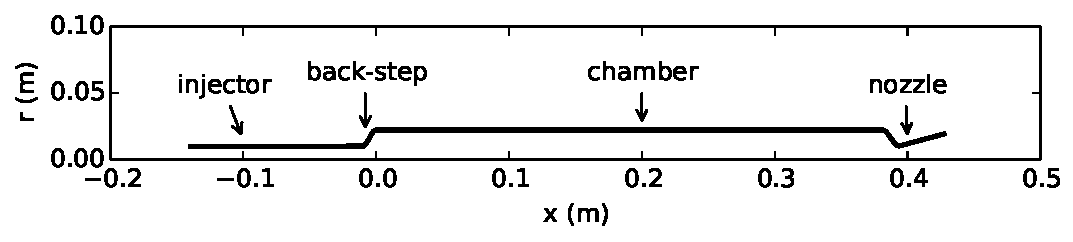
\includegraphics[width=0.8\linewidth]{pic/radius}
	\caption{Geometry of quasi-1D CVRC model.}
	\label{fig:radius}
\end{figure}

\begin{table} [h]
	\centering
	\caption{Geometry parameters of the quasi-1D CVRC with an oxidizer post length $L_{op}=14$ cm.}
	\centering
	\begin{tabular}{c c c c c c }
		\toprule
		\centering
		\multirow{2}{*}{Section} &
		\multicolumn{2}{c}{Oxidizer post} &
		\multirow{2}{*}{Chamber} &
		\multicolumn{2}{c}{Nozzle} \\
		\cmidrule(lr){2-3} \cmidrule(lr){5-6}
		& injector & back-step & & converging part & diverging part\\
		\midrule
		Length (cm) & 12.99 & 1.01 & 38.1 & 1.27 & 3.4 \\
		Radius (cm) & 1.02  & $1.02 \sim 2.25$ & 2.25 & $2.25 \sim 1.04$ & $1.04 \sim 1.95$ \\
		\bottomrule
		\label{tab:geometry_parameters}
	\end{tabular} 
\end{table}

The fuel is pure gaseous methane. The oxidizer is a mixture of 42\% oxygen and 58\% water (per unit mass). The oxidizer is injected in the oxidizer post at a temperature $T_{ox}=1030$ K so that both water and oxygen are in the gaseous phase. The operating conditions are listed in Table \ref{tab:operating-conditions}.

\begin{table} [h]
	\centering
	\caption{CVRC operating conditions.}
	\centering
	\begin{tabular}{l l l}
		\toprule
		\centering
		Parameter & Unit & Value \\
		\midrule
		Fuel mass flow rate, $\dot{m}_{f}$ & kg/s & 0.027   \\
		Fuel temperature, $T_{f}$ & K & 300   \\
		Oxidizer mass flow rate, $\dot{m}_{ox}$ & kg/s & 0.32   \\
		Oxidizer temperature, $T_{ox}$ & K & 1030   \\
		$O_2$ mass fraction in oxidizer, $Y_{O_2}$ & -- & 42.4\%   \\
		$H_2O$ mass fraction in oxidizer, $Y_{H_2O}$ & -- & 57.6\%   \\
		Mean chamber pressure & MPa & 1.34 \\
		Equivalence ratio, $E_r$ & -- & 0.8 \\
		\bottomrule
		\label{tab:operating-conditions}
	\end{tabular} 
\end{table}

For the combustion, we consider the one-step reaction model
\begin{equation*}\label{eq:combustion}
CH_4 + 2O_2 \rightarrow CO_2 + 2H_2O
\end{equation*}
We assume that the fuel reacts instantaneously to form products, allowing us to neglect intermediate species and finite reaction rates. As the equivalence ratio is less than one, there is oxidizer left after the combustion. Therefore, only two species need to be considered: oxidizer and combustion products.


The governing equations that describe the conservation of mass, momentum, and energy of the quasi-1D CVRC flow, are the quasi-1D unsteady Euler equations for multiple species, expressed in conservative form as
\begin{equation*}\label{eq:quasi-1D-equation}
\frac{\partial \mathbf{u}}{\partial t} + \frac{\partial \mathbf{f}}{\partial x} = \mathbf{s}_A + \mathbf{s}_f + \mathbf{s}_q.
\end{equation*}
The conserved variable vector $\mathbf{u}$ and the convective flux vector $\mathbf{f}$ are
\begin{equation*}\label{eq:CVRC-u-f}
\mathbf{u}= \left( \begin{gathered}
\rho A  \\
\rho uA  \\
\rho EA  \\
\rho Y_{ox} A \\
\end{gathered} \right), 
\mathbf{f} = \left( \begin{gathered}
\rho uA  \\
\left(\rho u^2 + p\right)A  \\
\left(\rho E + p\right)uA  \\
\rho uY_{ox} A \\
\end{gathered} \right),
\end{equation*}
where $\rho$ is the density, $u$ is the velocity, $p$ is the pressure, $E$ is the total energy, $Y_{ox}$ is the mass fraction of oxidizer, and $A=A(x)$ is the cross section area of the duct. The pressure $p$ can be computed using the conserved variables as
\begin{equation*}\label{eq:total-engery}
E = \frac{p}{\rho (\gamma - 1)} + \frac{u^2}{2} - C_p T_{ref},
\end{equation*}
where $T_{ref}$ is the reference temperature and is set as 298.15 K in this paper. The temperature $T$ is recovered from the equation of state $p = \rho R T$. The gas properties  $C_p$, $R$ and $\gamma$ are computed as $C_p= \sum C_{pi}Y_i$, $R=\sum R_iY_i$ and $ \gamma= C_p/(C_p-R)$, respectively. 

The source terms are
\begin{equation*}\label{eq:source-terms}
\mathbf{s}_A = \left( \begin{gathered}
0  \\
p \frac{dA}{dx}  \\
0  \\
0 \\
\end{gathered} \right), 
\mathbf{s}_f = \left( \begin{gathered}
{\dot \omega}_f  \\
{\dot \omega}_f u  \\
{\dot \omega}_f \left(h_{0}^{f} + \Delta h_{0}^{rel} \right)  \\
{\dot \omega}_{ox} \\
\end{gathered} \right), 
{\mathbf{s}_q} = \left( \begin{gathered}
0  \\
0  \\
q'  \\
0 \\
\end{gathered} \right),
\end{equation*}
where $\dot{\omega}_f$ is the depletion rate of the fuel, $\dot{\omega}_{ox}$ is the depletion rate of the oxidizer, $h_0^f$ is the total enthalpy of the fuel, $\Delta h_{0}^{rel}$ is the heat of reaction per unit mass of fuel and $q'$ is the unsteady heat release term. $\mathbf{s}_A$ accounts for area variations, $\mathbf{s}_f$ and $\mathbf{s}_q$ are related to the combustion. $\mathbf{s}_f$ represents the addition of the fuel and its combustion with the oxidizer, which in turn results in the creation of the combustion products. The depletion rate of the fuel is
\begin{equation}\label{eq:wf}
\dot{\omega}_{f}= \frac{k_f \dot{m}_f Y_{ox} \left(1+sin\xi\right)}{l_f-l_s},
\end{equation} 
where
\begin{equation*}\label{eq:xi}
\xi= -\frac{\pi}{2} + 2\pi\frac{x-l_s}{l_f-l_s}, \hspace{0.5cm} \forall \hspace{0.2cm} l_s < x < l_f.
\end{equation*}
The setting of the fuel injection restricts the combustion to the region $l_s < x < l_f$. The reaction constant $k_f$ is selected to insure that the fuel is consumed within the specified combustion zone. The depletion rate of the oxidizer is computed by 
\begin{equation*}\label{eq:wox}
\dot{\omega}_{ox} = C_{o/f} \dot{\omega}_f,
\end{equation*}
where $C_{o/f}$ is the oxidizer-to-fuel ratio.

The unsteady heat release term $q'$, also called the combustion response function, models the coupling between acoustics and combustion. In this paper, we use the combustion response function designed by Frezzotti et al. \cite{frezzotti2017numerical,frezzotti2018quasi}, which is a function of the velocity, sampled at specific abscissa $\hat{x}$ that is almost coincident with the antinode of the first longitudinal modal shape, with a certain time lag $\tau$, i.e.,
\begin{equation}\label{eq:response-function}
q'\left( x,t\right) = \alpha g\left(x\right)  A\left(x\right) \left[ u\left( \hat{x},t-\tau \right) - \bar{u}\left( \hat{x} \right) \right].
\end{equation}
Here $\bar{u}$ is the time averaged velocity, estimated with the steady-state quasi-1D model assuming $q'=0$, and $g(x)$ is a Gaussian distribution  
\begin{equation*}\label{eq:gx}
g\left(x\right)= \frac{e^{-\frac{\left(x-\mu\right)^2}{2\sigma^2}}}{\sqrt{2\pi\sigma^2}},
\end{equation*}
where $\mu$ is the mean and $\sigma$ is the standard deviation. The amount of heat release due to velocity oscillations is controlled by the parameter $\alpha$.

The boundary conditions for the quasi-1D CVRC flow include the fixed mass flow rate and the stagnation temperature at the head-end of the oxidizer injector, and the supersonic outflow at the exit of the nozzle.

Prior to unsteady simulation, the quasi-1D CVRC needs to be excited, which can be achieved by adding a perturbation to the steady-state solution. The perturbation is added by forcing the mass flow rate with a multi-sine signal
\begin{equation}\label{eq:multisine}
\dot{m}_{ox} \left(t\right)= \dot{m}_{ox,0} \left[1 + \delta\sum_{k=1}^{K}  sin\left(2\pi k\Delta f t\right) \right],
\end{equation}
where $\dot{m}_{ox,0}$ is the oxidizer mass flow rate in Table \ref{tab:operating-conditions}, $\Delta f$ is the frequency resolution and $K$ is the number of frequencies. In this paper, $\Delta f = 50 $ Hz and $K=140$, resulting in a minimal frequency of 50 Hz and a maximal frequency of 7000 Hz. $\delta$ is required to be small to control the amplitude of the perturbation and is set as 0.1\%.

The procedure of the unsteady simulation of the quasi-1D CVRC flow includes three steps:
\begin{enumerate}[(1)]
	\item  Compute the steady-state solution by setting $\dot{m}_{ox}=\dot{m}_{ox,0} $ and $q'=0$.
	\item  Excite the system by adding a perturbation to the oxidizer mass flow rate according to (\ref{eq:multisine}) and setting $q'=0$.
	\item  Perform the unsteady simulation by turning on the combustion response function $q'$ in (\ref{eq:response-function}) and turning off the oxidizer mass flow rate perturbation by setting $\dot{m}_{ox}=\dot{m}_{ox,0} $.	
\end{enumerate}


A high-fidelity quasi-1D CVRC flow solver is built by employing the MUSCL reconstruction \cite{delis1998tvd}, the Lax-Friedrichs flux \cite{shu1988efficient} and the strong stability preserving, three-stage Runge-Kutta (SSP RK3) time stepping \cite{jiang1996efficient}.
